\chapter{Politica de securitate}

Platforma \textit{MyBB} pune un accent foarte important pe securitate. Conform site-ului oficial, securitatea este cea mai mare proprietate. Cu toate acestea, dezvoltatorii sunt conștienți că orice e făcut de om este pasibil să conțină buguri / erori, de aceea au încercat să atragă utilizatorii să contribuie și ei la această latură. Au încercat să introducă un sistem de reward-uri, care la companiile mari se traduce în oferirea unei sume de bani în funcție de vulnerabilitatea submisă. Aici din păcate avem de-a face cu un proiect open source, un proiect în spate căruia nu există o companie, există doar ideea de voluntariat. Nu negăm că există o serie de oameni dispuși să doneze pentru o cauză, dar de multe ori aceste donații se reinvestesc în infrastructură în vederea menținerii proiectului online. Ca să nu o mai lungim foarte mult, cei care descoperă vulnerabilități și le raportează echipei MyBB vor fi trecuți pe o pagină onorifică a site-ului oficial - numită \textit{Security Hall of Fame}.

Este printre puținele platforme open source căreia i s-a făcut și un audit de securitate. Auditul a fost făcut în anul 2008, de către GulfTech. În urma acestui audit, s-a identificat câteva probleme și s-a putut trage concluzia că MyBB prezintă un low-risk record în ceea ce privește nivelul de securitate. Nici din punct de vedere istoric nu au fost găsite foarte multe high-risk vulnerabilități. De multe ori e important să înveți din greșeli, din problemele apărute de-a lungul timpului.

Tot de pe site-ul oficial - \textit{http://mybb.com}, se pot regăsi și câteva instrucțiuni pe care echipa MyBB le pune la dispoziție utilizatorilor. Până la urmă degeaba ai un sistem foarte sigur, dacă cei care îl administrează nu o fac corect. De aceea, trebuie cumva educați administratorii pentru a preîntâmpina diverse neplăceri mai târziu. Nu putem să le numim reguli. Ar fi doar niște recomandări. Le vom prezenta succint în paragrafele următoare.

\section{Actualizări periodice}

Utilizatorul trebuie să se asigure că are întotdeauna cea mai nouă versiune a platformei. Echipa MyBB este foarte proactivă și fixează o vulnerabilitate high-risk în cel mult 48 de ore. Numărul de actualizări pe an nu este foarte mare, o actualizare apare la un interval de 2-3 luni. Ce ar trebui să reținem aici? Faptul că actualizările sunt determinate în principiu de fixarea unei vulnerabilități importante sau introducea unui set major de feature-uri.

\section{Ascunderea versiunii platformei}

În ceea ce privește afișsarea versiunii curente a platformei, MyBB adoptă o politică diferită față de majoritatea competitorilor, în sensul în care în mod implicit versiunea platformei nu este afișată în subsol, alături de copyright. Cu cât cunoști mai puține lucruri despre un sistem, cu atât este mai greu să îl spargi. Asta nu înseamnă că administratorul nu are posibilitatea de a dezactiva acest comportament din panoul de administrare, dacă asta e ceea ce își dorește.

\section{Panoul de administrare}

Ca și majoritatea celorlalte platforme web, un forum oferă \textit{două interfețe}, o interfață de tip \textit{front-end} - forumul propriu-zis - unde predomină operațiunile de citire și un altă interfață de tipul \textit{back-end} - panoul de administrare - unde predomină operațiile de scriere. Din motive evidente, cea mai riscantă zonă din punct de vedere a securității o reprezintă cea de-a doua și anume panoul de administrare. O dată ce un utilizator a obținut acces la această zonă, el are control asupra întregului forum.

În acest sens, echipa MyBB ține să sublinieze faptul că panoul de administrare este doar pentru administratori. Celelalte grupuri de utilizatori nu au acces implicit la această zonă. Contează și numărul de administratori din sistem: \textbf{"More Admins = Less Security"}

Panoul de administrare trebuie ascuns, trebuie ținut la distanță de ceilalți utilizatori care nu au privilegii de administratori. De aceea ar fi bine să fie redenumit directorul în care se regăsesc sursele PHP pentru această zonă, din \textit{admin} în ceva mult mai bizar, folosind un string random. În acest caz, cel care pregătește un atac, sau are intenții mai puțin bune, trebuie să petreacă mai mult timp în descoperirea căii către panoul de administrare. Se poate merge și mai departe prin securizarea panoului de administrare folosind \textit{HTTP Basic Auth} cu o parolă adițională.

\subsection{Cod PIN}

\begin{wrapfigure}{r}{0.5\textwidth}
    \vspace{-60pt}
    \center{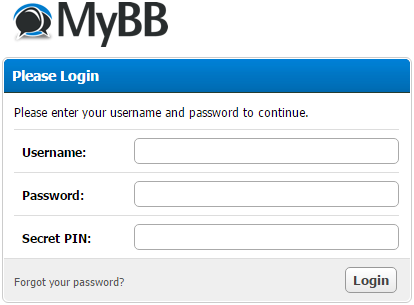
\includegraphics[width=0.5 \textwidth]{images/login.png}}
    \vspace{-20pt}
    \caption{\label{fig:Policy-AdminLogin} Autentificarea în AdminCP}
    \vspace{-10pt}
\end{wrapfigure}

Începând cu versiunea 1.8, în cadrul platformei s-a mai introdus un feature prin intermediul căruia se poate seta un cod PIN asupra panoului de administrare. Codul este format din 4 cifre și este static, putând fi modificat manual de administrator doar folosind accesul fizic la fișierele de configurare. Chiar dacă aduce un plus de securitate, prin cererea unor informații adiționale la autentificare, un dezavantaj ar fi faptul că acest cod nu se modifică automat după o perioadă de timp, modificările sale rămânând la latitudinea administratorului. În figura \ref{fig:Policy-AdminLogin} se poate observa existența acestui secret PIN.

\subsection{Backup-uri regulate}

Tot din panoul de administrare se poate configurare realizarea de backup-uri automate ale bazei de date la intervale periodice de timp. Procesul de backup este automatizat complet, arhiva rezultată putând fi păstrată pe server sau trimisă pe email, în cazul în care dimensiunea arhivei nu depășește 10 MB. Nu este necesar să facem un backup și la fișierele platformei pentru că acestea în mod normal ar trebui să fie recuperate ușor, fiind identice cu cele de pe site-ul oficial.

\section{Sistemul de modificări}

Platformei MyBB i se poate extinde funcționalitatea prin adăugarea unor modificări. Aceste modificări se numesc în termeni populari plugins. Sistemul de modificări funcționează prin intermediul interceptării unor evenimente ce au loc înainte sau după anumite acțiuni importante. Fiecare extensie, înregistrează la un dispatcher acțiunile pe care dorește să fie rulate atunci când un eveniment are loc. Așa după cum vă puteți da seama, fișierele de core nu sunt modificate sub nicio formă la instalarea unei noi modificări.

Comportamentul este puțin diferit față de ceea ce regăsim spre exemplu la platforma \textit{phpBB}, în care instalarea unei modificări presupune modificare unui sau mai multor fișiere din core. În cazul nostru, avantajul este reprezentat de faptul că fișierele de core rămân intacte, dezavantajul fiind introducerea unui overhead prin faptul că există un număr mai mare de apeluri de funcții. Se poate spune că securitatea este sporită în detrimentul performanței!

\newboxedtheorem[boxcolor=none, background=blue!5, titlebackground=blue!20, titleboxcolor = none]{theo}{Studiu de caz}{anything}
\begin{theo}[Număr de modificări utilizate]
Cu cât numărul de modificări instalate pe o platformă MyBB este mai mic cu atât riscurile în apariția unor vulnerabilități este mai mic. Momentan nu există o metodă prin care modificările realizate de către alți developeri să fie testate riguros, motiv pentru care acestea pot mai avea scăpări, introducând diverse probleme de securitate.\\
\textbf{Concluzie:} La ora actuală cele mai mari probleme de securitate au fost cauzate de tot felul de modificări.
\end{theo}

O să vedem un pic mai târziu ce face comunitatea oficială pentru a reduce numărul de modificări cu probleme de securitate.

\section{Controlul accesului în sistem}

Accesul în sistem se face prin intermediul unui mecanism simplu de autentificare pe baza unei parole și a unui nume de utilizator. Fiecare membru face parte dintr-un anumit grup de utilizatori și în funcție de grupul din care face parte, are un anumit set de permisiuni.

Grupurile de utilizatori implicite, care sunt create automat o dată cu instalarea platformei, sunt: administratorii, moderatorii, super moderatorii, membrii, vizitatorii și utilizatorii banați. Dintre aceștia doar administratorii au acces implicit la panoul de administrare. Există și noțiunea de super administrator, dacă ar fi să facem o analogie cu un sistem Linux, ar fi un utilizator root. Diferența dintre un simplu administrator și un super admin este constituită în principal din ideea că administratorii simplii nu au dreptul să modifice setul de permisiuni al unui super admin. Tot din motive de securitate, pentru membrii din staff (și anume moderatori, super moderatori și administratori), permisiunile pot fi setate și indivual pentru fiecare membru în parte. Există atât permisiuni la nivel de group cât și permisiuni individuale.

\begin{wrapfigure}{l}{0.5\textwidth}
    \vspace{-10pt}
    \center{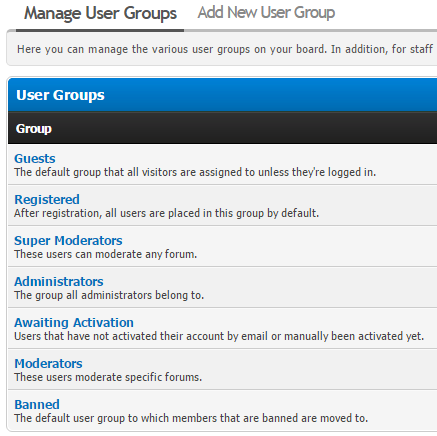
\includegraphics[width=0.5 \textwidth]{images/groups.png}}
    \vspace{-20pt}
    \caption{\label{fig:Policy-Groups} Grupurile preexistente}
    \vspace{-10pt}
\end{wrapfigure}

Cu cât sunt mai puțini administratori în sistem cu atât riscul compromiterii unui astfel de cont este mai mic, iar forumul este mai sigur. În plus, fiecare membru din staff ar trebui să primească un număr minimal de permisiuni, strict ceea ce are nevoie pentru a-și desfășura activitatea. Este sugerată aplicarea unei tactici de tipul "divide and conquer" în momentul în care există mai mulți membri în staff. Asta înseamnă că dacă un membru este specializat pe partea de design, atunci acesta ar trebui să primească permisiuni numai la această secțiune, fără a avea acces la setări, utilizatori sau utilitarele de sistem.

Una dintre cele mai importante neajunsuri în ceea ce privește grupurile de utilizatori, o reprezintă faptul că la autentificarea utilizatorului nu se face și o verificare mai amănunțită a IP-ului pe care utilizatorul îl folosește. Nu este corelată zona cu IP-ul folosit. Există o modificare care permite o astfel de corelare, ce are rolul de a bloca utilizatorii care se autentifică azi dintr-o țară (precum România) și după câteva ore din altă țară, dar funcționalitatea nu este implementată direct în core.

\section{Filtrarea informației}

Platforma acordă un deosebit interes în filtrarea informațiilor pe care utilizatorul le poate introduce în sistem ca și input. În mod implicit, codul HTML nu este permis în mesajele și subiectele ce sunt publictate în comunitate. Acest lucru este prezent și pentru celelalte formulare pe care platforma le pune la dispoziție. Cu toate acestea, dacă administratorul dorește în mod explicit să permită inserarea de cod HTML în diverse pagini, o poate face prin diferite setări ale aplicației. El trebuie să știe totuși că se predispune la un risc important din punct de vedere al securității.

\section{Sesiuni și parole}

Imediat după ce s-a realizat procesul de autentificare, fiecarui utilizator i se creează o sesiune pentru o perioadă de timp, astfel încât la următoarea pagină vizitată să nu mai fie nevoit să se autentifice în sistem, să mai introducă încă o dată credențialele. Perioada de timp poate fi atât temporară cât și pe termen nelimitat. Din motive de securitate evidente, sesiunea este corelată atât cu o serie de informații cu privire la browser-ul pe care îl folosește utilizatorul. Ca și principiu de funcționare, în momentul în care autentificarea s-a realizat cu succes se crează o nouă intrare într-o tabelă cu sesiuni, specificată utilizatorului respectiv pentru o perioadă de timp, după care utilizatorului i se setează un cookie cu câteva informații despre sesiunea respectivă (\textit{uid} și \textit{loginkey}). Sesiunea este ștearsă fie când a expirat, fie când se produce delogarea utilizatorului în mod explicit.

\begin{wrapfigure}{l}{0.6\textwidth}
    \vspace{-10pt}
    \center{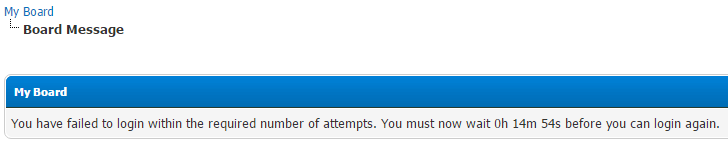
\includegraphics[width=0.6 \textwidth]{images/attempts.png}}
    \vspace{-20pt}
    \caption{\label{fig:Policy-FailedAttempts} Blocarea utilizatorului}
    \vspace{-10pt}
\end{wrapfigure}

Pentru a evita atacurile de tip brute-force, prin incercarea repetată a introducerii unor credențiale, există un mecanism prin care după un anumită de autentificări eșuate utilizatorului nu îi mai este permisă autentificarea. După 10 autentificări consecutive eșuate, utilizatorul este banat timp de 15 minute. Partea ce mai proastă legat de acest mecanism o reprezintă implementarea, care se bazează tot pe cookie-uri. Numărul de autentificări eșuate și data ultimei autentificări de acest gen sunt păstrate în două cookie-uri separate. În acest fel, dacă setăm browser-ul să nu păstreze cookie-urile sau le ștergem după fiecare autentificare eșuată, vom putea trece de acestă barieră.

Pentru accesarea panoului de administrare este necesară o sesiune diferită. Asta înseamnă că o dată ce ne-am autentificat în pagina de index, nu avem acces implicit și la panoul de administrare fără o altă validare a credențialelor. Per total această funcționalitate este bună, prin prisma introducerii unei verificări adiționale. Se putea face ceva mai bine, prin ștergerea sesiunii destinate panoului de administrare de fiecare dată când utilizatorul părăsește panoul de administrare, așa cum se întâmplă la platforma \textit{Woltlab}.

În ceea ce privește procesul de înregistrare, acesta este destul de simplu, neavând condiții foarte complexe pentru setarea acesteia. Condiția implicită pentru declararea unei parole ca fiind acceptată este să aibă minim 6 caractere ca și lungime. Cu toate acestea, platforma pune la dispoziția administratorilor, o setare prin care poate activa verificarea parolei pentru a deveni ceva mai complexă. O dată activată această setare, fiecare parolă ce va fi setată sau schimbată va trebui să aibă cel puțin 6 caractere ca și lungimr, să conțină cel puțin o cifră, o literă mare și una mică.

Ca și un alt fapt divers, platforma presupune că adresa de email a utilizatorului este intangibilă, fiind cel mai important instrument prin care se poate valida autenticitatea unui membru. De aceea, acest instrument este folosit pentru recuperarea parolelor pierdute sau semnarea unor decizii pe care utilizatorul trebuie să le ia în cadrul comunității.

\section{Interacțiunea cu comunitatea oficială}

Comunitatea oficială pune la dispoziția utilizatorilor săi o serie de informații cu privire la modul în care platforma poate fi utilizată, aducând laolaltă toți internauții ce o folosesc pentru propria comunitate. Oamenii găsesc aici tot felul de noutăți, recomandări, tutoriale și articole despre diverse teme cât și o serie de modificări și teme pe care le pot folosi pentru a customiza forumul personal.

Din perspectiva unui developer, adică a unui om ce contribuie la dezvoltarea comunității și a platformei lucrurile stau puțin diferit. Spuneam undeva prin paragrafele anterioare că modificările sunt cele care cresc probabilitatea de a aduce vulnerabilități în propria comunitate. Echipa MyBB a decis să nu oblige administratorii de forumuri să instaleze extensii doar de pe site-ul oficial. Astfel, extensiile (fie că vorbim de modificări sau teme) pot fi instalate și dintr-o sursă locală, prin încărcarea unei arhive pe server. Acest comportament nu este din păcate ideal, pentru că sunt o serie de modificări ce pot fi instalate fără să fie împrealabil verificate de o serie de persoane autorizate. Și nu vorbim de o reacredință din partea contributorilor, doar că există probabilitatea ca cel care a dezvoltat respectivul plugin să nu aibă experiența necesară, să fie începător și să nu ia toate măsurile necesare pentru securitatea extensiei sale.

Din fericire, sistemul implementat pe site-ul oficial permite verificarea materialelor încărcate și testarea minimă a acestora. O dată încărcat un astfel de material, există o serie de utilitare ce verifică fișierele sursă pentru a vedea dacă sunt vulnerabile diferitor tipuri de atacuri, gen SQL Injection sau XSS. Dacă totul este în regulă, o persoană autorizată din echipa se va uita manual peste modificare și va fi cea care va da acceptul final pentru publicarea materialului. De asemenea, un sistem de rating și de raportare a problemelor cu diverse extensii permite rezolvarea rapidă a vulnerabilităților sau dezactivarea extensiei dacă autorul ei nu dorește să fixeze problemele evidențiate de alți utilizatori.